\chapter[Sistema Eletrônico]{Sistema Eletrônico}

Explicação da estruturação do texto do sistema eletrônico

\section{Sistema de sensoriamento da estação}

	A produtividade de uma cultura pode ser ampliada a partir do controle das mais diversas variáveis do ambiente. O conhecimento de tais parâmetros possibilita ao produtor criar condições mais favoráveis ao desenvolvimento da plantação. As estações desenvolvidas no projeto RICC serão capazes de medir as seguintes grandezas:

	\begin{itemize}
		\item Referentes ao ambiente externo:
		\begin{enumerate}
			\item Umidade relativa do ar
			\item Temperatura do ar
			\item Pressão atmosférica
			\item Velocidade e direção do vento
			\item Pluviosidade
			\item Radiação solar
		\end{enumerate}	 		
	
		\item Referentes ao solo:	
		\begin{enumerate}
			\item Umidade
			\item Temperatura
		\end{enumerate}	
	\end{itemize}

	As medições internas do solo fornecem informações mais específicas sobre o estado da plantação e o seu desenvolvimento. Por exemplo, a temperatura do solo tem impacto no processo de germinação das plantas, afetando sua aquisição de nutrientes e absorção de água \cite{bib_sen_01_jose}.	

	Já a umidade do solo trata do dado mais significativo para o projeto, pois é o que permite efetivamente o controle da irrigação. Nessa linha, diversos trabalhos estudaram o desenvolvimento de um sistema de controle automático da irrigação \cite{romero2012research} \cite{zhao2009study}, onde medições são realizadas em regiões separadas da plantação, realimentando um sistema de controle da bomba para a manter a taxa de umidade do solo dentro de um intervalo predeterminado e relacionado ao tipo de cultura. No nosso projeto, serão realizadas medições em três níveis, pois o ponto ideal de medição da umidade do solo depende do tamanho da raíz e das características de absorção da planta \cite{su2014critical}.

	A diversidade dos aspectos do solo, como sua composição de grãos e presença de sais minerais, influencia diretamente na dinâmica hídrica. Ou seja, o comportamento da infiltração e do escoamento superficial da água são próprios do solo em monitoramento \cite{bib_sen_01_ian}. Para a validação desse trabalho optamos por um solo característico da região do Distrito Federal, retirado da Fazenda Água Limpa (FAL) da UnB, onde existe a disponibilidade de dois tipos de solo característicos:

	\begin{itemize}
		\item Latossolo vermelho amarelo; solo argiloso (composição de argila igual ou superior a $30\%$), menos permeável, apresenta grande capacidade de armazenar água.
		\item Neossolo; solo arenoso (composição de argila igual ou inferior a $15\%$ e de areia superior a $70\%$) onde o escoamento da água no solo é acelerado.    
    \end{itemize}	

    Os dados coletados para o ambiente externo são de extrema importância para a agricultura, pois permitem a modelagem do processo de evapotranspiração, o que caracteriza os ciclos de água e de energia do ecossistema, além de contribuir para a análise e previsão das condições climáticas \cite{bib_sen_04_victor}. Informações sobre o comportamento desse processo na plantação podem embasar tomadas de decisões agrícolas como: a escolha do período para cultivo, colheita ou plantação \cite{bib_sen_05_victor}; a gestão do processo de irrigação \cite{bib_sen_06_victor}; a antecipação de condições erráticas do clima \cite{bib_sen_07_victor}.

	As medidas do ambiente externo e do solo serão utilizadas no controle de irrigação de forma complementar, o que será melhor detalhado nas próximas seções. Para cada grandeza a ser medida, serão especificados o processo de escolha do sensor, o condicionamento do sinal, a necessidade de calibração e o algoritmo de processamento. 

	\subsection{Cálculo da evapotranspiração}

		Neste projeto, os dados climáticos serão utilizados com foco na gestão do processo de irrigação e por meio da modelagem da evapotranspiração em plantações de soja no solo do Cerrado. O estudo dessa modelagem, nas condições especificadas para o projeto, foi realizado pela Embrapa \cite{bib_sen_01_victor} e será usado como base para o trabalho. 

		Dessa forma, a evapotranspiração será calculada de acordo com o método de Penman-Monteith, padrão indicado pela FAO (\emph{Food and Agriculture Organization}) \cite{bib_sen_02_victor}. Baseado nesse estudo, podemos estimar a evapotranspiração da cultura em milímetros de água durante o intervalo de medição $\delta$ ($mm/\delta$), como sendo:

		\begin{eqnarray}
			Et_c = K_c.Et_o
		\end{eqnarray}
		onde $K_c$ é o coeficiente da cultura e $Et_o$ é a evapotranspiração de referência em $mm/\delta$. O coeficiente da cultura $K_c$  será calculado usando a curva ajustada em \cite{bib_sen_03_victor}, pela seguinte equação:

		\begin{eqnarray}
			K_c = -0,00022x^2 + 0,0318x + 0,4588
		\end{eqnarray}
		sendo que $x$ é a quantidade de dias após a emergência da planta e será determinado pela data de emergência, a qual deverá ser especificada pelo produtor por meio da interface do aplicativo. 

		Já a evapotranspiração de referência em $mm \delta ^{-1}$ pode ser definida pelo método de Penman-Monteith como:

		\begin{eqnarray}
		Et_{o}=\dfrac {0,408\Delta\left( R_{n}-G\right) +\gamma \dfrac {900}{T+273}u_2\left( e_{s}-e_{a}\right) }{\Delta +\left( 1+0,34u_2\right) }
		\end{eqnarray}
		em que:
		\begin{itemize}
			\renewcommand{\labelitemi}{$\Rightarrow$}
			\item $R_n$: saldo de radiação à superfície ($MJ m^{-2}/\delta$).
			\item $G$: fluxo de calor no solo ($MJ m^{-2}/\delta$).
			\item $T$: temperatura do ar na altura da estação ($^{\circ}C$).
			\item $u_2$: velocidade do vento à 2 metros de altura ($m/s$).
			\item $e_s$: pressão de saturação de vapor (kPa).
			\item $e_a$: pressão atual do vapor (kPa).
			\item $\Delta$: declividade da curva de pressão de saturação de vapor ($kPa/^{\circ}C$).
			\item $\gamma$: constante psicométrica ($kPa/^{\circ}C$).
		\end{itemize}
		
		As variáveis $R_n$ e $T$ serão estimadas usando, respectivamente, as medições dos sensores de radiação solar e temperatura do ar, os quais serão descritos posteriormente. Sabendo que a velocidade do vento pode mudar em função da altura, e que altura do sensor será inferior à 2 metros, uma correção será aplicada, conforme especificado em \cite{bib_sen_08_victor}. Dessa forma, a velocidade do vento à 2 metros $u_2$ será estimada como:

		\begin{eqnarray}
			u_2 = u_{z}\dfrac {4,87}{\ln \left( 67,8z-5,42\right)}
		\end{eqnarray}
		onde $z = 1,15m$ é a altura de medição e $u_z$ é a velocidade do vento medida nessa altura.

		De acordo com \cite{bib_sen_08_victor}, o fluxo de calor no solo $G$ é aproximadamente zero para medições diária, ou seja, $\delta = 1$ dia. Já para medições horárias ou em períodos menores é possível fazer a aproximação $G=0,1 R_n$ durante o dia e $G=0,5 R_n$ durante a noite. Por esse motivo, a determinação de $G$ será realizada em função da horário da medição e da periodicidade $\delta$ definida.

		Além disso, a pressão de saturação de vapor $e_s$ pode ser definida em função da temperatura do ar $T$, a partir da equação: (trocar pela equação do matão)

		\begin{eqnarray}
			e_s = 0,6108 \exp \left[ \frac {17,27T}{T+237.3}\right]
		\end{eqnarray}
		e a pressão atual do vapor $e_a$ pode ser estimada por $e_s$ e pela umidade relativa do ar (em $\%$) $UR$, que será medida pelo sensor de umidade do ar, de acordo com a seguinte equação:

		\begin{eqnarray}
			e_s = \frac {UR.e_s}{100}
		\end{eqnarray}
		
		O declividade da curva de pressão de saturação de vapor $\Delta$ também pode ser calculado em função da temperatura do ar $T$, como sendo:

		\begin{eqnarray}
			\Delta = \frac {4098\left[ 0,6108\exp \left( \frac {17,27T}{T+237,3}\right) \right] }{\left[ T+237,3\right] ^{2}}
		\end{eqnarray}
		
		Por fim, a constante psicométrica $\gamma$ pode ser calculado como:

		\begin{eqnarray}
			\gamma = A.P
		\end{eqnarray}
		onde A é o coeficiente psicrômetro com ventilação natural ($80x10^{-5}/^{\circ}C$) e $P$ é a pressão atmosférica em $kPa$ que será estimada pelo sensor de pressão do ar.

	\subsection{Umidade relativa, temperatura e pressão do ar}

		Seguindo a trabalho realizado no ponto de controle 1, o grupo havia decidido pelo uso do sensor DHT22 para realizar as medições de umidade relativa e temperatura do ar. A escolha se deu com base nos critérios de disponibilidade, custo (um mesmo sensor para mais de uma medição desejada) e a faixa de operação (quando comparado com o modelo DHT11). 

		Entretanto, como consequência da decisão de calcular a evapotranspiração da plantação, veio a necessidade de medição da pressão atmosférica e, com isso, os sensores do ambiente externo tiveram que ser reavaliados de forma a procurar uma melhor solução para o sensoriamento. Após uma pesquisa rápida, foi encontrado o sensor BME280, o qual realiza a medição de pressão atmosférica em conjunto com as medições de umidade relativa e temperatura do ar, sendo então um potencial substituto para o sensor DHT22.

		\subsubsection{Escolha do sensor}
		Com o intuito de avaliar o desempenho do sensor BME280 quando comparado com o sensor DHT22, foi realizado uma tabela listando as características operacionais de ambos com relação às medições de temperatura e umidade relativa, tabela \ref{tab_ele_victor_02}.

		\begin{table}[]
			\centering
			\caption{Comparação entre os sensores para umidade relativa e temperatura}
			\label{tab_ele_victor_02}
			\begin{tabular}{|c|c|c|c|c|c|c|}
				\hline
				\begin{tabular}[c]{@{}c@{}}Sensor de\\ umidade e \\ temperatura\end{tabular} & \begin{tabular}[c]{@{}c@{}}Faixa de \\ operação\\ (\%RH)\end{tabular} & \begin{tabular}[c]{@{}c@{}}Resolução\\ (\%RH)\end{tabular} & \begin{tabular}[c]{@{}c@{}}Acurácia\\ (\%RH)\end{tabular} & \begin{tabular}[c]{@{}c@{}}Faixa de \\ operação\\ (°C)\end{tabular} & \begin{tabular}[c]{@{}c@{}}Resolução\\ (°C)\end{tabular} & \begin{tabular}[c]{@{}c@{}}Acurácia\\ (°C)\end{tabular} \\ \hline
				DHT22 & 0 - 100 & 0,1 & ± 5 & -40 - 80 & 0,1 & ± 0,5 \\ \hline
				BME280 & 0 - 100 & 0,008 & ± 3 & -40 - 80 & 0,01 & ± 1,0 \\ \hline
			\end{tabular}
		\end{table}

		Segundo os dados coletados, o sensor com maior acurácia é o SHT30, contudo é a opção mais cara. O sensor DHT11, apesar de ser o menos custoso, tem uma faixa de operação reduzida e a diferença de preço é pequena em comparação com o DHT22. Contudo, por um pequeno aumento de custo, o sensor BME280 apresenta uma melhor acurácia e menor consumo de corrente. Além disso, este último também realiza medições de pressão atmosférica e temperatura do ar, grandezas necessárias para o cálculo de evapotranspiração. Por esse motivo e pela maior vantagem financeira (com relação ao SHT33), o sensor escolhido é o BME280. Como esse sensor apresenta uma resolução ($0,008\%RH$) em escala consideravelmente menor que sua acurácia ($\pm 3 \%RH$), será considerada uma variação mínima de $0,1\%RH$ durante o processamento.

		\begin{table}[]
			\centering
			\caption{Comparação entre os sensores de pressão atmosférica}
			\label{tab_ele_victor_pre}
			\begin{tabular}{|c|c|c|c|}
				\hline
				\begin{tabular}[c]{@{}c@{}}Sensor de\\ pressão\end{tabular} & \begin{tabular}[c]{@{}c@{}}Faixa de\\ operação\\ (hPa)\end{tabular} & \begin{tabular}[c]{@{}c@{}}Resolução\\ (hPa)\end{tabular} & \begin{tabular}[c]{@{}c@{}}Acurácia\\ (°C)\end{tabular} \\ \hline
				BMP280 & 300 - 1100 & 0,01 & ± 1,0 \\ \hline
				BME280 & 300 - 1100 & 0,18 & ± 1,0 \\ \hline
			\end{tabular}
		\end{table}

		\begin{table}[]
			\centering
			\caption{Comparações gerais entre os sensores avaliados para umidade relativa, temperatura e pressão do ar.}
			\label{tab_ele_victor_bm}
			\begin{tabular}{|c|c|c|c|c|c|}
				\hline
				Sensor & \begin{tabular}[c]{@{}c@{}}Tensão de\\ entrada \\ (V)\end{tabular} & \begin{tabular}[c]{@{}c@{}}Consumo de\\ corrente \\ (mA)\end{tabular} & Comunicação & \begin{tabular}[c]{@{}c@{}}Pinos de \\ comunicação\end{tabular} & \begin{tabular}[c]{@{}c@{}}Preço \\ (R\$)\end{tabular} \\ \hline
				DHT22 & 3,3 - 6 & 1,5 & Serial & 2 Digitais & 34,99 \\ \hline
				BMP280 & 1,8 - 3,6 & 1,0 & I2C & 2 Digitais & 42,70 \\ \hline
				BME280 & 1,71 - 3,6 & 0,714 & I2C & 2 Digitais & 33.35 \\ \hline
			\end{tabular}
		\end{table}

		\subsubsection{Condicionamento do sinal}

		Neste caso, nenhum condicionamento é necessário para o sinal, pois isso já é realizado internamente no módulo. Dessa forma, a conexão com o microcontrolador pode ser realizada diretamente pela linhas SDA e SCL e pela alimentação Vin e Gnd. O sensor escolhido comunica seus dados pelo protocolo I2C e já converte as medições para suas respectivas unidades: $\% RH$ para umidade relativa do ar,  $\circ C$ para temperatura do ar e $hPa$ para a pressão atmosférica. 

		\subsubsection{Calibração}

		Apesar dessas medidas não necessitarem de uma calibração para conversão de unidade, os fabricantes recomendam um processo de compensação para melhorar a acurácia da medida. Esse processo consiste na extração de parâmetros salvos nos registradores do módulo, que são usados em uma função (disponível no \emph{datasheet}) para corrigir os valores medidos.

		\subsubsection{Algoritmo de processamento}

		O algoritmo de processamento para este sensor está exemplificado no pseudocódigo \ref{alg_ele_victor_01}

		\begin{center}
			\begin{minipage}{0.5\linewidth} % Adjust the minipage width to accomodate for the length of algorithm lines
				\begin{algorithm}[H]
					\label{alg_ele_victor_01}
					\KwIn{$(a, b)$, two floating-point numbers}  % Algorithm inputs
					\KwResult{$(c, d)$, such that $a+b = c + d$} % Algorithm outputs/results
					\medskip
					\If{$\vert b\vert > \vert a\vert$}{
						exchange $a$ and $b$ \;
					}
					$c \leftarrow a + b$ \;
					$z \leftarrow c - a$ \;
					$d \leftarrow b - z$ \;
					{\textbf return} $(c,d)$ \;
					\caption{\texttt{FastTwoSum}} % Algorithm name
					\label{alg:fastTwoSum}   % optional label to refer to
				\end{algorithm}
			\end{minipage}
		\end{center}

	\subsection{Velocidade e direção do vento}

		\subsubsection{Escolha do sensor}

		O equipamento mais comum de medição da velocidade do vento é o anemômetro. Esse instrumento converte a força eólica em movimento rotacional. A velocidade do vento está relacionada à velocidade angular deste movimento. Dentre o modelos de anemômetro existentes, os de copo destacam-se pela simplicidade de construção e eficiência de conversão do movimento, sua configuração se assemelha à de um gerador eólico com quatro pás no rotor.

		Foram encontrados poucos modelos disponíveis no mercado brasileiro, porém seus valores elevados ( a partir de R$\$ 139,98$, para modelos simples) inviabilizaram o uso no projeto. Levando em consideração a facilidade de construção de um anemômetro de copo e, sobretudo, com o intuito de reduzir os custos , foi  decidido inicialmente pela construção desse sensor. Dessa forma, a estrutura seria projetada e impressa em 3D. A velocidade angular seria medida por meio da interação de sensores de efeito hall  com imãs posicionados no rotor.

		Pelos mesmos motivos apresentados para o anemômetro, também optou-se pela construção do sensor de direção do vento. Porém, neste caso, utiliza-se uma haste horizontal e uma bandeira, de forma que a força do vento fará com que a haste se alinhe com sua direção. Para determinar a direção da haste, uma configuração de sensor hall também com um imã de neodímio pode ser utilizada. 
		
		O professor Alex Reis disponibilizou ao grupo o equipamento 034B da empresa \emph{Met One Instruments} figura \ref{ele_sen_gab_01}, que é formado pelos sensores de velocidade e direção do vento. Seu valor de venda de US$\$~785,00$  foi encontrado no site \url{https://www.stevenswater.com}. Uma vez que este instrumento trata-se de um modelo comercial desenvolvido para uso em estações meteorológicas, optou-se por seu uso no lugar dos equipamentos que projetaríamos. A acurácia obtida nas medições é de $\pm 4^{\circ}$ para direção e de $\pm 0,1 m/s$, e a resolução é de $0,5^{\circ}$ para direção 
		
		\begin{figure}
			\centering
			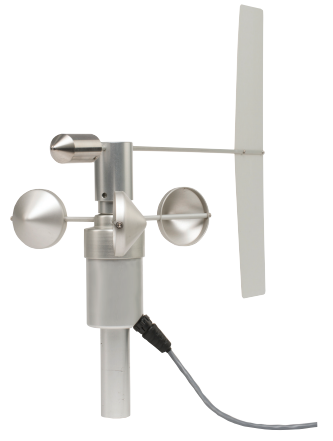
\includegraphics[width = 0.3\textwidth]{sensores/figuras/ele_pc2_gab_01}
			\caption{Sensor 034B. Fonte: \cite{bib_sen_gab_01}}
			\label{ele_sen_gab_01}
		\end{figure}
		
		Os princípios de funcionamento do sensor 034B são semelhantes aos descritos anteriormente. Para a determinação de velocidade há um \emph{Reed Switch} (chave acionada magneticamente), por onde são gerados pulsos a uma frequência relacionada à velocidade do vento. Este valor de frequência $f_{Hz}$ em Hertz será lido no microcontrolador e convertida para uma velocidade $V_{mps}$ em $m/s$  por meio da equação seguinte, fornecida pelo fabricante no manual de operação do sensor \cite{bib_sen_gab_02}.
		
		\begin{equation}
			V_{mps} = \frac{f_{Hz}}{1,2517} + 0,28	
		\end{equation}
		
		A direção do vento é determinada com o auxílio de um potenciômetro linear. Será portanto, montado um divisor de tensão resistivo. A direção é proporcional à queda de tensão que for observada. O manual de operação recomenda que seja associado um resistor de $1 k \Omega$ para evitar sobrecarga no equipamento.
		
		Dado o elevado custo do sensor que será usado para a construção do protótipo, buscamos possíveis substitutos menos onerosos para utilização no projeto de um possível produto final. Este componente deve ter o maior número de características compatíveis com o utilizado. Assim, garante-se que as soluções propostas neste trabalho continuem válidas, ou que sejam minimamente modificadas.
		
		O anemômetro produzido pela empresa brasileira WRF Comercial possui o mesmo princípio de funcionamento e pode ser alimentado com os mesmos valores de tensão. Assim, as conexões físicas e algoritmos mantem-se os mesmos em ambos os casos. Entretanto, os processos de calibração e confiabilidade dos dados devem ser reavaliados, já que o fabricante não fornece informações suficientes para que se faça previamente tais inferências. Essas informações foram requisitadas ao fabricante, porém não obtivemos resposta até o momento. Para o produto final, uma solução viável seria a construção dos sensores, como descrito no começo desta seção.

		\subsubsection{Condicionamento do sinal}

		\subsubsection{Calibração}

		\subsubsection{Algoritmo de processamento}

	\subsection{Pluviosidade}

		No primeiro ponto de controle, foi detalhado o processo de escolha do sensor de pluviosidade, avaliando sensores comerciais, sensores de chuva e a fabricação de um sensor. Os sensores de chuva foram descartados devido a necessidade de impermeabilização e maior sucestibilidade à ruídos do meio. Em relação aos sensores comerciais, não foi encontrado uma opção viável para o projeto e, portanto, decidiu-se pela fabricação do pluviômetro. Este sensor seria realizado no modelo de gangorra e usando um sensor de efeito Hall para realizar a medição. 

		Entretanto, assim como para o sensor de velocidade e direção do vento, o professor Alex Reis emprestou ao grupo um pluviômetro comercial modelo TB4 da \emph{Hydrological Services America} (HSA) figura \ref{ele_sen_vic_01}.

		\begin{figure}[H]
			\centering
			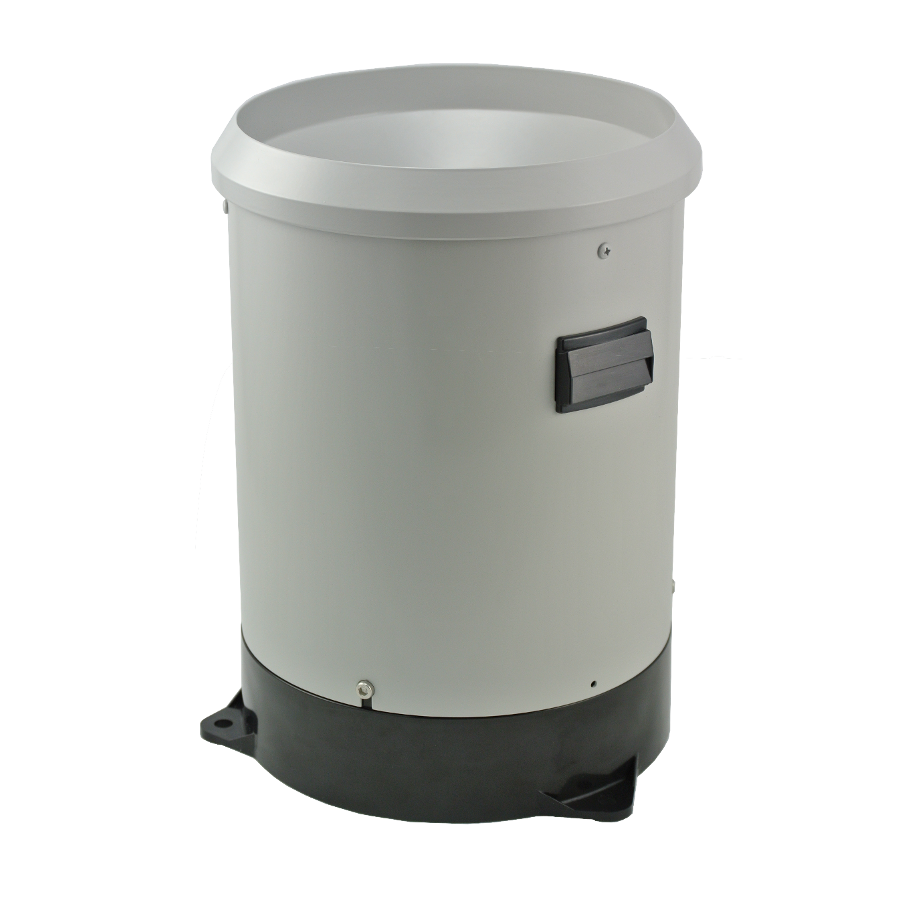
\includegraphics[width = .35 \textwidth]{sensores/figuras/ele_sen_vic_01}
			\caption{Pluviômetro TB4 pela HSA. Fonte: \cite{bib_sen_vic_01}}
			\label{ele_sen_vic_01}
		\end{figure}

		\subsubsection{Definição do sensor}

		O pluviômetro comercial da HSA foi encontrado anunciado pela empresa Fondriest por um preço de $US\$ 850,00$ sem taxas de entrega, o que se converte em aproximadamente $R\$ 3140,00$ (pela conversão atual de 3,92). Esse preço excede o limite previsto para o projeto e, portanto, não seria uma solução viável para o produto final. 

		Contudo, apesar de não ser uma opção viável financeiramente, ainda é possível ser usado como prova de conceito no protótipo. Isso porque outros sensores mais simples, como o fornecido pela empresa brasileira WRF Comercial (por $R\$ 148,50$) apresentam o mesmo princípio de funcionamento e dimensões semelhantes. 

		Mais especificamente, ambos os sensores funcionam usando \emph{Reed Switches} em conjunto com imãs fixados na estrutura e na mesma configuração de gangorra descrita anteriormente. Por esse motivo, a lógica do programa de processamento desse sinal poderia ser mantida, apenas necessitando de uma nova calibragem. As informações de comparação entre os sensores está descrita na tabela \ref{tab_sen_vic_03}

		\begin{table}[H]
			\centering
			\begin{miniscule}
				\caption{Comparação entre os sensores de pluviosidade do fabricantes avaliados.}
				\label{tab_sen_vic_03}
				\begin{tabular}{|c|c|c|c|c|c|c|c|c|c|}
					\hline
					Fabricante & \begin{tabular}[c]{@{}c@{}}Faixa de\\ operação \\ (mm/hr)\end{tabular} & \begin{tabular}[c]{@{}c@{}}Resolução \\ (mm)\end{tabular} & \begin{tabular}[c]{@{}c@{}}Acurácia \\ (\%mm)\end{tabular} & \begin{tabular}[c]{@{}c@{}}Tensão de\\ entrada \\ (V)\end{tabular} & Comunicação & \begin{tabular}[c]{@{}c@{}}Pinos\\ (A/D)\end{tabular} & \begin{tabular}[c]{@{}c@{}}Diâmetro\\ (mm)\end{tabular} & \begin{tabular}[c]{@{}c@{}}Altura\\ (mm)\end{tabular} & \begin{tabular}[c]{@{}c@{}}Preço\\  (R\$)\end{tabular} \\ \hline
					WRF & - & 0,25 & - & - & Analógica & 1 A & 147 & 160 & 148,50 \\ \hline
					HSA & 0 - 700 & 0,2 & ± 3 & 0 - 12 & Analógica & 1 A & 200 & 315 & 3140,00 \\ \hline
				\end{tabular}
			\end{miniscule}
		\end{table}

		Analisando a tabela \ref{tab_sen_vic_03}, percebe-se que a diferença nas dimensões entre os sensores é alta, porém, o sensor fabricado pela WRF possui ambas as dimensões de altura e diâmetro menores, possibilitando o projeto de uma estrutura de adaptação mais simples para o encaixe.

		O problema deste último sensor da WRF está em sua falta de documentação, a qual foi requisitada para o fabricante, sem resposta até o momento de escrita deste documento. Assim, no caso de ausência de informação, as métricas de faixa de operação e acurácia devem ser testadas experimentalmente. Ainda, pensando em um produto a longo prazo, seria interessante a fabricação deste sensor (como planejado anteriormente) para reduzir os custos do produto.

		Os dados de consumo de corrente destes sensores dependem do circuito de condicionamento, considerando que são compostos apenas de chaves magnéticas passivas. Uma vez escolhido o sensor TB4 da empresa HSA para o protótipo, foi definido o circuito de condicionamento da mesma forma que o circuito da figura \ref{}, por se tratarem de \emph{Reed Switches} com mesmo propósito

		\subsubsection{Condicionamento do sinal}

		O circuito de condicionamento deste sensor pode ser com apenas um resistor de \emph{pull-down}

		\subsubsection{}

		O processo de calibração deste sensor envolve o conhecimento prévio das dimensões do funil e das características mecânicas da gangorra interna. Essas características se encontram no \emph{datasheet} do sensor e são, mais especificamente, 

		\subsubsection{Algoritmo de processamento}

		O algoritmo de processamento previsto para este sensor está exemplificado no pseudocódigo \ref{alg_ele_victor_01}

		\begin{center}
			\begin{minipage}{0.5\linewidth} % Adjust the minipage width to accomodate for the length of algorithm lines
				\begin{algorithm}[H]
					\label{alg_ele_victor_01}
					\KwIn{$(a, b)$, two floating-point numbers}  % Algorithm inputs
					\KwResult{$(c, d)$, such that $a+b = c + d$} % Algorithm outputs/results
					\medskip
					\If{$\vert b\vert > \vert a\vert$}{
						exchange $a$ and $b$ \;
					}
					$c \leftarrow a + b$ \;
					$z \leftarrow c - a$ \;
					$d \leftarrow b - z$ \;
					{\textbf return} $(c,d)$ \;
					\caption{\texttt{FastTwoSum}} % Algorithm name
					\label{alg:fastTwoSum}   % optional label to refer to
				\end{algorithm}
			\end{minipage}
		\end{center}

	\subsection{Radiação solar}

		   

	\subsection{Umidade do solo}
		 
	A medição de umidade do solo é central para o projeto e, portanto, deve ser definida criteriosamente. Dentre as formas de medição encontradas para essa aplicação, foram separadas no primeiro ponto de controle três categorias de sensores que cumprem as restrições de custo e disponibilidade: tensiômetros, sensores resistivos e sensores capacitivos. Ainda no ponto de controle 1, foi decidido pelo uso de sensores capacitivos, devido à melhor relação entre acurácia de medição, durabilidade, disponibilidade e custo.
	
		\subsubsection{Definição do sensor}
		
		Dentre os sensores capacitivos encontrados, o que melhor se adequou ao projeto foi o sensor SoilWatch 10 da empresa Pino-Tech (figura \ref{soil_sen_03}). Esse sensor é completamente a prova d'água e já foi usado em projetos de controle de irrigação, sendo ideal para a nossa aplicação.

		\begin{figure}[H]
			\centering
			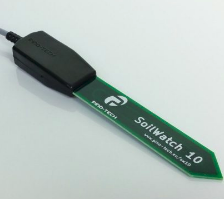
\includegraphics[width = .5 \textwidth]{sensores/figuras/soil_sen_03}
			\caption{Soil Watch 10 sensor de umidade do solo. Fonte: \cite{bib_soil_sen_03}}
			\label{soil_sen_03}
		\end{figure}	

		Entretanto, este sensor ainda não é disponível no Brasil e o custo de importação seria muito alto para o projeto, além do risco associado ao tempo de entrega. Por esse motivo, foi decidido deixar esse sensor como ideia para um produto futuro e foram avaliadas outras possibilidades mais viáveis para o protótipo. Dentre as possibilidades destacou-se o sensor SEN0193 (figura \ref{soil_sen_02}) pelos critérios de custo e documentação disponível, já que para a maior parte dos sensores avaliados nenhuma documentação específica foi encontrada. Dessa forma, esse foi o sensor escolhido para o protótipo.
		
		\begin{figure}[H]
			\centering
			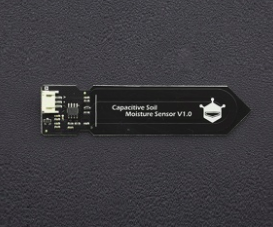
\includegraphics[width = .5 \textwidth]{sensores/figuras/soil_sen_02}
			\caption{Sensor de umidade do solo modelo SEN0193. Fonte: \cite{bib_soil_sen_02}}
			\label{soil_sen_02}
		\end{figure}	
		
		De forma a analisar as mudanças que seriam necessárias para a transição do sensor SEN0193 para o sensor Soil Watch 10, pensando em um produto final, foi montada a tabela \ref{ele_sen_victor_05} com os parâmetros operacionais de ambos. Pela tabela vemos que as tensões de entrada e saída assim como a faixa de operação são diretamente compatíveis. Houve apenas um pequeno aumento no consumo de corrente e variações nas dimensões físicas. Em relação as dimensões, da forma que foi pensada a estrutura seriam necessárias poucas alterações, apenas uma adaptação no encaixe do medidor. Apesar do sensor SEN0193 não ser completamente a prova d'água, a parte com circuito exposta será isolada pela estrutura do medidor.

		\begin{table}[H]
		\centering
		\caption{Comparação entre os sensores de umidade do solo capacitivos}
		\label{ele_sen_victor_05}
			\begin{miniscule}
				\begin{tabular}{|c|c|c|c|c|c|c|c|c|c|}
				\hline
				Fabricante & \begin{tabular}[c]{@{}c@{}}Faixa de\\ operação \\ (\%RH)\end{tabular} & \begin{tabular}[c]{@{}c@{}}Tensão de\\ entrada\\  (V)\end{tabular} & \begin{tabular}[c]{@{}c@{}}Tensão de\\ saída \\ (V)\end{tabular} & \begin{tabular}[c]{@{}c@{}}Consumo de\\ corrente \\ (mA)\end{tabular} & Comunicação & \begin{tabular}[c]{@{}c@{}}Pinos\\ (A/D)\end{tabular} & \begin{tabular}[c]{@{}c@{}}Largura\\ (mm)\end{tabular} & \begin{tabular}[c]{@{}c@{}}Altura\\ (mm)\end{tabular} & \begin{tabular}[c]{@{}c@{}}Preço \\ (R\$)\end{tabular} \\ \hline
				DFRobot & 0 - 100 & 3,3 - 5,5 & 0 - 3 & 5 & Analógica & 1 A & 23 & 98 & 29,90 \\ \hline
				Soil Watch & 0 - 100 & 2,8 - 5,0 & 0 - 3 & 24 & Analógica & 1 A & 25 & 170 & 85,14 \\ \hline
				\end{tabular}
			\end{miniscule}
		\end{table}

		\subsubsection{Condicionamento do sinal}

		O condicionamento do sinal deste sensor é realizado internamente no módulo, de forma a produzir na saída um sinal analógico proporcional à capacitância medida. Assim, o sensor pode ser conectado diretamente na entrada analógica do microcontrolador, produzindo um número inteiro digital de 0 a 1023. Porém, esse número ainda não representa um valor real de umidade.

		\subsubsection{Calibração}

		Devido a sensibilidade do sensor quanto as características do ambiente, a obtenção de valores reais de umidade depende do tipo de solo e da cultura escolhida. Assim, para garantir que a leitura analógica do sensor esteja de acordo com o valor efetivo de umidade do solo, é necessário um processo de calibração. 
		
		Basicamente, devemos ajustar as saídas dos sensores capacitivos de acordo com alguma medição de referência. A prática de calibração (calibragem) ocorre predominantemente em duas situações, a calibragem em solo, no local de controle da irrigação e a calibragem em laboratório, realizada em ambiente controlado. Nosso contato com a Faculdade de Agronomia e Medicina Veterinária e com a Embrapa Hortaliças, constatou que ambas praticam a calibragem em laboratório, tendo em vista a dificuldade de preparação do processo em solo. Além disso, a Embrapa Hortaliças se disponibilizou a auxiliar no processo fornecendo orientação e infraestrutura local para a prática desse trabalho. Justificando assim nossa escolha por esse modelo.
		
		A ideia geral da prática é recolher uma amostra de solo em um recipiente controlado (cuja a massa é conhecida/medida) monitorando a massa do conjunto solo-recipiente, processo conhecido como gravimetria. Assim, saturando a amostra de solo com água, acompanhar as medições dos sensores junto da variação da massa total. Para associar esses valores de massa à uma umidade de referência é necessário secar em estufa o conjunto a fim de obter a massa seca total. A umidade gravimétrica em um instante $t$ é dada por \cite{bib_sen_02_ian}:
		
		\begin{align*}
			\textsc{U}(t) &= \frac{m_{su}(t)-m_{s}}{m_{s}} 
		\end{align*}
		
		Onde $m_{su}(t)$ é a massa de solo úmido em um instante $t$ e $m_{s}$ é a massa de solo seco (lembrando que o valor da massa do recipiente deve ser descontado dessas medidas). A metodologia do procedimento (extraída de \cite{bib_sen_01_ian}, \cite{bib_sen_02_ian} e \cite{bib_sen_03_ian}) é descrita a seguir:
		
		\begin{itemize}
			\item Materiais e ferramentas:

			\begin{itemize}
				\item Sensores de umidade capacitivos;
				\item Amostra do solo do cultivo (a altura do perfil da amostra depende da cultura);
				\item Recipiente vazado para evasão de água;
				\item Microcontrolador para tratamento de dados;
				\item Sensor de temperatura;
				\item Balança de precisão.
			\end{itemize}

		\item Procedimentos:

			\begin{enumerate}
				\item Recortar e fazer a retirada do perfil do solo para calibração de acordo com a cultura a ser monitorada;
				\item Retirar resquícios orgânicos e minerais (plantas e pedras) do solo;
				\item Secar em estufa o solo a uma temperatura de $105 \degree C$ durante um período de pelo menos $24$ horas;
				\item Medir a massa do recipiente vazio $m_0$;
				\item Posicionar junto ao solo a estrutura do sensor no recipiente a uma altura desejada de medição de acordo com a cultura;
				\item Medir a massa do conjunto seco $m_s+m_0$;
				\item Testar a estabilidade dos sensores; irrigar até o ponto de saturação do solo e realizar medições ao longo de um período de $20$ minutos com amostragem de $1$ coleta por minuto. 
				\item Monitorar a temperatura ambiente e do recipiente;
				\item Saturar o solo com água;
				\item Posicionar o conjunto solo-recipiente na balança para determinar a massa umida saturada $m_{su}(0)+m_0$;
				\item Calcular o valor de referência da umidade gravimétrica $U(0)$;
				\item Retirar o conjunto da balança e repousar em temperatura ambiente, garantindo a evasão da água do solo;
				\item Realizar medições do sensor capacitivo em um período de $1$ horas com taxa de atualização de $1$ amostra por minuto;
				\item Após o intervalo de $1$ hora, reposicionar o conjunto na balança determinando a massa úmida $m_{su}(1)+m_0$;
				\item Calcular o valor de referência da umidade gravimétrica $U(1)$;
				\item Repetir o processo de secagem e pesagem em intervalos de $1$ hora, computando a umidade gravimétrica junto as medições do sensor capacitivo até que o valor da \textit{k-ésima} medida seja inferior a uma cota relacionada ao tipo de solo e cultura específica $U(k) \leq \alpha$. 
			\end{enumerate}	

		\end{itemize}
		
		 Algumas considerações são necessárias para esse método. Em primeiro lugar, realizar a calibragem para cada sensor envolvido nas medições, além de repetir o processo para acúmulo de dados e garantir precisão estatística para a coleta. Além disso, relacionar os valores obtidos pela gravimetria com os dados dos sensores capacitivos, utilizando um método estatístico de minimização do erro quadrático.
		 
		 Esse processo pode ser refinado, principalmente em relação a grandeza de referência, garantindo uma maior precisão para os sensores. Substituindo a análise da umidade gravimétrica $U(t)$ pela umidade volumétrica $\theta(t)$, acrescentamos mais um parâmetro de controle das características do sistema, a densidade do solo $\rho_s$ \cite{bib_sen_01_ian}. A umidade volumétrica é definida por:

		 \begin{align*}
		 	\theta(t) &= U(t) \rho_s = \frac{m_{su}(t)-m_{s}}{m_{s}} \rho_s
		 \end{align*}
		
		Até o presente momento a viabilidade do monitoramento da densidade do solo não foi aferida, podendo ou não entrar no procedimento de calibração.
		
		O $\alpha$ é um valor de umidade gravimétrica mínimo obtido de uma umidade volumétrica $\theta_{min}=0,100~m^3 m^{-3}$ \cite{bib_sen_01_ian}. Para a conversão necessitamos do valor da densidade do solo, o que pode ser consultado da seguinte tabela extraída de \cite{bib_sen_04_ian}:
		
		\begin{table}[H]
			\caption{Características do solo para diferentes texturas}
			\label{CSDT}
			\begin{tabular}{|l|l|l|l|}
				\hline
				Textura do Solo & Densidade $\rho_s$ & Cc ($\%$ em peso) & DTA ($mm/cm$) \\ \hline
				Arenosa & 1,55 - 1,80 & 10 - 20 & 0,6 - 1,0 \\ \hline
				Franco-arenosa & 1,40 - 1,60 & 15 - 27 & 0,9 - 1,5 \\ \hline
				Franco-arenosa-argilosa & 1,35 - 1,50 & 11 - 17 & 1,4 - 2,0 \\ \hline
				Franco-argilosa & 1,30 - 1,40 & 31 - 42 & 1,6 - 2,2 \\ \hline
				Argilosa & 1,20 - 1,30 & 39 - 49 & 2,0 - 2,5 \\ \hline
			\end{tabular}
		\end{table} 	    
		
		Onde Cc representa a capacidade de campo, ponto de saturação do solo, e DTA a Disponibilidade Total de Água do Solo segundo \cite{bib_sen_04_ian}. Além dessa forma, podemos medir a densidade do solo escolhido, determinando mais precisamente o valor de $\alpha$. Por fim:
		\begin{align*}
		\alpha &= \frac{\theta_{min}}{\rho_s} = \frac{0,100}{\rho_s} \Rightarrow 0,055 \leq \alpha \leq 0,084
		\end{align*}

		\subsubsection{Algoritmo de processamento}

		\begin{center}
			\begin{minipage}{0.5\linewidth} % Adjust the minipage width to accomodate for the length of algorithm lines
				\begin{algorithm}[H]
					\label{alg_ele_victor_01}
					\KwIn{$(a, b)$, two floating-point numbers}  % Algorithm inputs
					\KwResult{$(c, d)$, such that $a+b = c + d$} % Algorithm outputs/results
					\medskip
					\If{$\vert b\vert > \vert a\vert$}{
						exchange $a$ and $b$ \;
					}
					$c \leftarrow a + b$ \;
					$z \leftarrow c - a$ \;
					$d \leftarrow b - z$ \;
					{\textbf return} $(c,d)$ \;
					\caption{\texttt{FastTwoSum}} % Algorithm name
					\label{alg:fastTwoSum}   % optional label to refer to
				\end{algorithm}
			\end{minipage}
		\end{center}

	\subsection{Temperatura do solo}

		São vários os materiais transdutores que podem ser utilizados para medição de temperatura: termopares, termistores, termorresistências e junções PN. É importante que o sensor escolhido possua um encapsulamento que suporte as condições de maiores umidade e corrosividade.

		\subsubsection{Escolha do Sensor}

		Abaixo estão relacionados alguns possíveis sensores comerciais que atendem as necessidades do projeto em termos de faixa de operação e acurácia da medida. 


		\begin{table}[H]
		\centering
		\caption{Possíveis sensores para temperatura do solo}
		\label{tab_ele_gab_02}

		\begin{tabular}{|c|c|c|c|c|c|c|}
		\hline
		Sensor & \begin{tabular}[c]{@{}c@{}}Faixa de\\ operação \\ ($^{\circ}C$)\end{tabular} & \begin{tabular}[c]{@{}c@{}}Acurácia \\ ($^{\circ}C$)\end{tabular} & \begin{tabular}[c]{@{}c@{}}Tensão de\\ entrada\\  ($V$)\end{tabular} & \begin{tabular}[c]{@{}c@{}}Consumo de\\ corrente\\ ($mA$)\end{tabular} & \begin{tabular}[c]{@{}c@{}}Preço\\ ($R\$$)\end{tabular} & Pinos \\ \hline
		LM35 & $-55$ - $150$ & $\pm 0,5$ & 4 - 30 & 60 & 8,91 & 1 analógico \\ \hline
		Ds18b20 & $-55$ - $125$ & $\pm 0,5$ & 3 - 5 & 1 & 12,99 & 1 digital \\ \hline
		Pt100 & $-200$ - $650$ & $\pm 0,1$ & 3 - 5 & - & 10,96 & 1 analógico \\ \hline
		\end{tabular}

		\end{table}

		Todas as opções levantadas possuem uma ampla faixa de operação, que contempla a esperada para temperatura do solo. Os preços são  semelhantes, fazendo com que o principal critério de escolha seja a acurácia. Neste caso, a melhor opção é o Pt100. 

		O consumo de corrente para o Pt100 depende do circuito que o condiciona, visto que trata-se de uma resistência que varia em função da temperatura, por isso tal valor não é encontrado na tabela \ref{tab_ele_gab_02}.  

		\subsubsection{Condicionamento do Sinal}
			A resistência $R_T$ do Pt100 a uma temperatura $T$ é conseguida por meio da seguinte equação, onde $R_0 = 100~\Omega$ é a resistência do sensor a $0^{\circ}C$. 
				
			\begin{equation}
			R_T = R_0 (1 + 3,9083 \cdot 10^{-3} T)
			\end{equation}

		Portanto, a resistência $R_T$ deve ser medida para que se calcule a temperatura $T$. Para tanto, foram levantados dois possíveis circuitos, apresentados na figura \ref{ele_pc2_gab_02}


			\begin{figure}
				\centering
				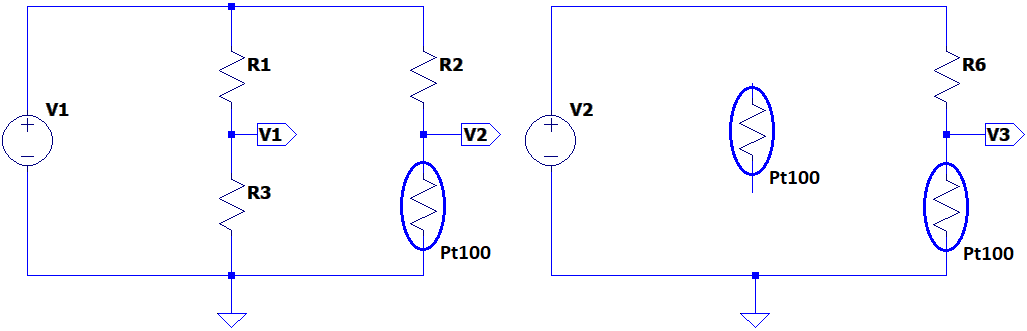
\includegraphics[width = .7 \textwidth]{sensores/figuras/ele_pc2_gab_02}
				\caption{Circuitos de condicionamento para Pt100}
				\label{ele_pc2_gab_02}
			\end{figure}

		O primeiro circuito, apresentado à esquerda, é uma ponte de Wheatstone, que quando em equilíbrio não apresenta diferença de potencial entre os nós $V_1$ e $V_2$. As variações de resistência no Pt100 fazem com que haja uma tensão observável entre estes nós, a partir da qual é estimada a resistência $R_T$ e obtida a temperatura $T$. Ainda, é necessária a amplificação deste sinal para que possa ser entendido pelo microprocessador.

		O segundo circuito, apresentado à direita, é um divisor de tensão. A queda de tensão vista no Pt100 é proporcional a sua resistência, e deste modo também é possível estimar o valor desejado da temperatura $T$.

		Ambos os circuitos foram simulados utilizando o software LTspice para que se pudesse avaliar suas performances. A amplificação necessária para a ponte de Wheatstone foi executada com um INA128 (seu modelo de simulação é fornecido no site de seu fabricante, Texas Instruments). O Pt100 foi simulado como uma resistência variando entre $109~\Omega$ e $119~\Omega$, correspondendo aproximadamente às temperaturas $24^{\circ}C$ e $49^{\circ}C$, respectivamente.

		\subsubsection{Calibração}

		\subsubsection{Algoritmo de processamento}


\section{Sistema de Comunicação}
		
\subsection{Especificação do Transceptor RF}

Essa seção se dedica a especificação do módulo RF a ser utilizado, tratando sobre os protocolos de comunicação das camadas OSI (\emph{Open System Interconnection}) já implementadas. O padrão OSI  é um modelo de rede de computadores amplamente utilizado em aplicações de telecomunicações. Trata-se de uma arquitetura para protocolos de comunicação. O modelo secciona redes de computadores em sete camadas, com objetivo de que a cada camada seja atribuída uma funcionalidade assinalada por um protocolo específico. As sete camadas do sistema OSI são: Física, Enlace, Rede, Transporte, Sessão, Apresentação e Aplicação. Nesta sessão vamos tratar mais especificamente das camadas Física e de Enlace, que são as implementadas no módulo RF nRF24LE1.

\subsubsection{Camada Física}

Na camada física são tratados os seguintes parâmetros: (i) taxas de transferência de dados, (ii) frequência de recepção e de transmissão, (iii) largura de banda do sinal e (iv) filtros de recepção. O módulo RF nRF24LE1, implementa a camada física, sendo o objetivo deste documento apresentar suas características.

O módulo RF nRF24L01p, opera no espectro ISM (\emph{Industrial, Scientific and Medical}) que possui banda de operação entre $2,4~GHz$ e $2,4835GHz$, possui modulação GFSK, interface de antena comum no transmissor e receptor e taxas de transmissão de dados $250~Kbps$, $1~Mbps$ e $2~Mbps$. A seguir é mostrado o diagrama de blocos do transceptor.

\begin{figure}[H]
\centering
	\label{com_pc2_01}
	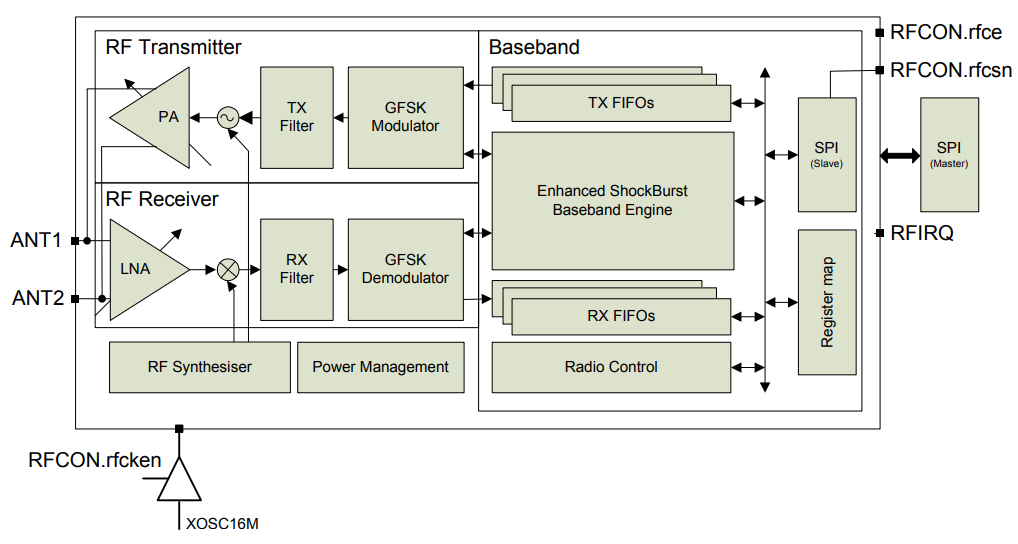
\includegraphics[width= .8\textwidth]{sensores/figuras/com_pc2_01.png}
   \caption{Diagrama de Blocos Transceptor RF. Fonte: \cite{bib_com_01_yas}}
\end{figure}

%\paragraph*{Modos de Operação}
O transceptor possui um máquina de estados que controla os diferentes modos de operação, são eles:  (i)\emph{Power Down}, (ii)\emph{Standby-I}, (iii) \emph{Standby-II}, (iv) RX e (v)TX. A seguir é mostrada a máquina de estados do transceptor e uma descrição de cada um deles. 


\begin{itemize}

	\item[(i)] \emph{Power Down}: O transceptor RF é desabilitado com consumo mínimo de corrente. Todos os valores dos registradores disponíveis pelo SPI são mantidos e o SPI pode ser ativado.
	\item[(ii)] \emph{Standby-I}: Usado para minimizar o consumo médio de corrente e manter tempos curtos de inicialização. O modo ativo ocorre somente se o bit rfce (\emph{control enable}) estiver ativado, enquanto não estiver, o transceptor de RF retorna ao Standby-I dos modos TX e RX.
	\item[(iii)] \emph{Standby-II}: Nesse modo os \emph{buffers} de \emph{clock} extras são ativados e há maior consumo de corrente em comparação com ao (ii). O transceptor de RF entrará no modo de espera II se o bit rfce for mantido alto durante uma uma transmissão com os FIFOs de transmissão (FIFOs TX) vazio. Se um novo pacote é baixado para o FIFO TX, o filtro PLL é iniciado imediatamente e o pacote é transmitido após o atraso normal de estabelecimento do PLL ($\delta t _ {PLL} = 130 \mu s$).
	\item[(iv)] RX: Transceptor é ativado como receptor. Nesse modo, o receptor demodula os sinais que chegam no canal, apresentando constantemente os dados demodulados ao mecanismo de protocolo de banda base. Se um pacote válido for encontrado (por um endereço correspondente e um CRC()válido), o \emph{payload} do pacote será apresentado em um \emph{slot} livre nos FIFOs de recepção (FIFOs RX). Se os FIFOs RX estiverem cheios, o pacote recebido é descartado.
	O transceptor permanece nesse modo até o microcontrolador configurar os modos (i) ou (ii). Entretanto se o protocolo de enlace(Enhanced ShockBurst\texttrademark) estiver habilitado, o transceptor pode assumir outros modos para executar o protocolo.
	\item[(v)] TX: Transceptor é ativado como transmissor e permanece ativo até que não haja mais pacotes a serem transmitidos nos FIFOs TX, se o bit rfce estiver alto, caso contrário o modo TX fica ativo até finalizar a transmissão de um pacote apenas. é importante nunca deixar o transceptor em modo TX por mais de $4~ms$ por vez. Se o protocolo de enlace estiver ativado, o modo TX nunca fica ativo por mais de $4~ms$.
\end{itemize}


\begin{figure}[H]
\centering
	\label{com_pc2_02}
	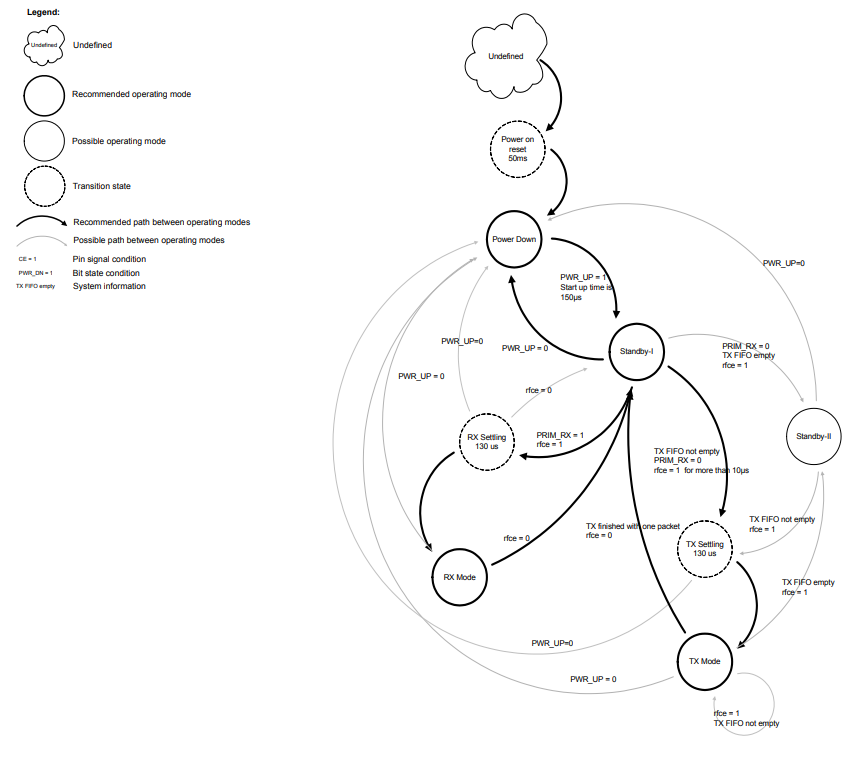
\includegraphics[width=\textwidth]{sensores/figuras/com_pc2_02.png}
   \caption{Máquina de Estados dos Modos de Operação do Transceptor RF. Fonte: \cite{bib_com_01_yas}}
\end{figure}

Na tabela \ref{tab_com_pc1_01} é apresentada as configuração dos registradores para cada modo de operação da máquina de estados.

\begin{table}[H]
\caption{Modos de operação}
\label{tab_com_pc1_01}
\begin{tabular}{|c|c|c|c|c|}
\hline
Modo & \begin{tabular}[c]{@{}c@{}}Registrador\\ PWR-UP\end{tabular} & \begin{tabular}[c]{@{}c@{}}Registrador\\  PRIM\_ RX\end{tabular} & rfce & Estado dos FIFOs \\ \hline
RX & 1 & 1 & 1 & - \\ \hline
TX & 1 & 0 & 1 & \begin{tabular}[c]{@{}c@{}}Esvazia todos os níveis \\ no FIFO $\text{TX}^a$\end{tabular} \\ \hline
TX & 1 & 0 & \begin{tabular}[c]{@{}c@{}}Mínimo de $10\mu s$\\  de pulso alto\end{tabular} & \begin{tabular}[c]{@{}c@{}}Esvazia apenas um nível \\ no FIFO $\text{TX}^b$\end{tabular} \\ \hline
Standby-I & 1 & 0 & 1 & FIFO TX vazio \\ \hline
Standby-II & 1 & - & 0 & \begin{tabular}[c]{@{}c@{}}Sem pacotes para \\ transmissão a caminho\end{tabular} \\ \hline
Power Down & 0 & - & - & - \\ \hline
\end{tabular}

\begin{flushright}
\begin{tiny}
a - Se o bit rfce é mantido alto o FIFO TX é esvaziado e todos os ACK necessários e possíveis retransmissões são realizados. A transmissão continua enquanto o FIFO TX for recarregado. Se o FIFO de TX estiver vazio quando o bit rfce ainda estiver alto, o transceptor de RF entrará em Standby-II. Neste modo, a transmissão de um pacote é iniciada assim que o rfce é definido alto após o \emph{upload} de um pacote para o FIFO TX.

b - Este modo de operação realiza um pulso alto no bit rfce por pelo menos $10~\mu s$ . Permitindo a transmissão de um único pacote. Este é o modo de operação normal, e após a transmissão do pacote, o transceptor de RF entra no Standby-I.
\end{tiny}
\end{flushright}
\end{table}

\paragraph*{Frequência do Canal}
A largura de banda ocupada por cada canal depende da taxa de transmissão usada no transceptor. Para as taxas de $250~kbps$ e $1~Mbps$, a largura de banda será inferior a $1~MHz$. Entretanto, se usada uma taxa de $2~Mbps$, a largura do canal pode atingir até $2~MHz$. Isso significa que a frequência central dos diferentes canais devem estar espaçadas em, pelo menos, $1~MHz$ nos primeiros casos e $2~MHz$ no último, para garantir que não haverá sobreposição. Para o transceptor escolhido, o mínimo espaçamento programável (resolução da frequência do canal) é de $1~MHz$.


A frequência do canal é inicializada pelo registrador RF\_{CH} de acordo com a fórmula 
$F_0= 2400 + \text{RF\_{CH}}~MHz$
Para comunicação mútua, o receptor e o transmissor devem ter a mesma frequência do canal RF.

\paragraph*{Detector de Potência Recebida (RPD)}

O RPD, localizado no bit 0 do registrador 9, dispara a partir de níveis de potência acima de -64 dBm detectados no canal, caso contrário o RDP = 0.

O RPD pode ser lido a qualquer momento enquanto o transceptor RF estiver em modo RX. Isso oferece um \emph{snapshot} do nível atual de potência recebida no canal. O RPD é bloqueado sempre que um pacote é recebido ou 
quando o microcontrolador define rfce = 0. O status do RPD está correto quando o modo RX está ativado e após um tempo de espera de \emph{Tstby2a + Tdelay\_ AGC} = 130us + 40µs. O ganho de RX varia com a temperatura, o que significa que o limiar de RPD também varia temperatura. O \emph{threshold} de RPD é reduzido em 5dB a $T = -40^{\circ}C$ e aumentado em 5dB a $85 ^{\circ}C$.

\subsubsection{Camada de Enlace}

Na camada de Enlace, o módulo RF nRF24LE1 possui o protocolo Enhanced ShockBurst\texttrademark. O protocolo consiste em uma camada de enlace baseada em pacotes de dados que apresenta montagem automática dos pacotes,
temporização, reconhecimento automático (\emph{ack}) e retransmissões de pacotes. O Enhanced ShockBurst\texttrademark permite a implementação de comunicação de baixo consumo de energia e alto desempenho.

%\paragraph*{Características do Enhanced ShockBurst\texttrademark}

As principais cateterísticas do protocolo são:
\begin{itemize}
\item Entre 1 e 32 \emph{bytes} de comprimento de \emph{payload};
\item Manuseio de pacotes automático
\item Manuseio das transações de pacotes automático
	\item \emph{Ack} automático
	\item Retransmissão automática
\end{itemize}

%\paragraph*{\emph{Overview} do Enhanced ShockBurst\texttrademark}

Como dito anteriormente, o Enhanced ShockBurst\texttrademark ~ possui temporização e manuseio de pacote automático. Como o protocolo consiste em um enlace de dados bidirecional, ou seja, é uma comunicação ponto a ponto consistindo em dois transceptores, um Receptor Primário (\emph{PRX}) e um Transmissor Primário (\emph{PTX}). O protocolo sempre é iniciado e finalizado no transmissor, a partir da transmissão do pacote e ao fim da transação com um pacote \emph{ack} recebido pelo transmissor. 

É importante ressaltar que o Enhanced ShockBurst\texttrademark ~ possibilita a configuração do número máximo de retransmissões e o \emph{delay} máximo entre as retransmissões. Todo o manuseio automático do protocolo é feito sem o microcontrolador. 

\paragraph*{Formato do pacote do Enhanced ShockBurst\texttrademark}

\begin{figure}[H]
\centering
	\label{com_pc2_03}
	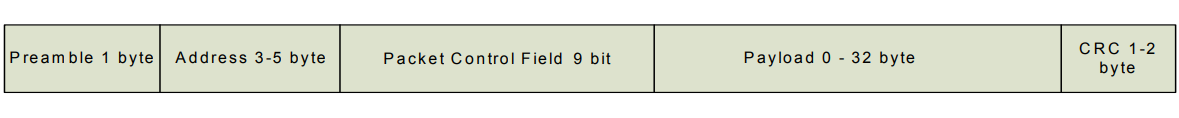
\includegraphics[width=\textwidth]{sensores/figuras/com_pc2_03.png}
   \caption{Formato do Pacote do Enhanced ShockBurst\texttrademark}
\end{figure}

\begin{itemize}
	\item Preâmbulo (\emph{preamble}): é responsável pela sincronização do demodulador no receptor para receber a sequência de bits que estão chegando. Esse procedimento é feito para estabilizar o receptor.
	\item Endereço (\emph{Address}): Este é o endereço do destinatário. O endereço garante que o pacote correto seja detectado pelo receptor. 
	\item Campo de Controle do Pacote (\emph{Packet Control Field}): Neste campo contém um campo de 6 bits para indicar o tamanho do pacote, um campo de 2 bits com a \emph{ID} do pacote para identificar se é um pacote novo ou uma retransmissão e um bit para um \emph{flag} de \emph{no-ack}.
	\item \emph{Payload}: O \emph{Payload} é a carga útil do pacote e é um conteúdo definido pelo usuário do pacote. Pode ter de 0 a 32 bytes de largura.
	\item \emph{CRC - (Cyclic Redundancy Check)}: O CRC é o mecanismo de detecção de erros no pacote. Pode ter 1 ou 2 bytes e é calculado sobre o Endereço, Campo de Controle do Pacote e Payload. Se o CRC falhar o pacote não é aceito pelo Enhanced ShockBurst\texttrademark.
\end{itemize}

\subsection{Algoritmo da Rede de Comunicação}


O protocolo já estabelecido do módulo nRF24L01 define a camada de enlace garantindo o fluxo de dados a uma taxa confiável para comunicação ponto a ponto. Assim, faz-se necessária a implementação de uma rede de comunicação em malha. De modo a  prover uma comunicação estável entre duas estações que não estejam diretamente conectadas, procurando um caminho possível através de outras estações.

Essa comunicação é baseada no padrão IEEE 802.11s \cite{bib_ele_du_1}, que estabelece um padrão flexível e extensível de comunicação para redes wireless Ad-Hoc em malha \cite{bib_ele_du_5}. A figura \ref{ele_pc2_du_01} apresenta a organização dessa rede, onde MP são pontos de malha, basicamente nós comuns com recursos de malha, MAPs são pontos de acesso de malha e MPPs são pontos de malha com função de portal.

\begin{figure}[H]
\centering
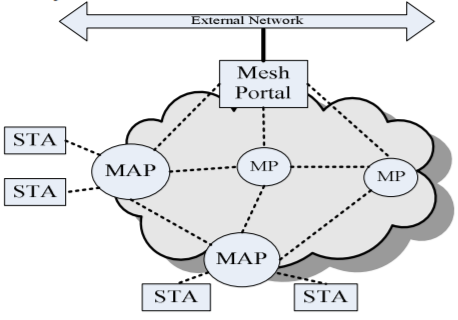
\includegraphics[width=.5\textwidth]{sensores/figuras/ele_pc2_du_01}
\caption{Rede mesh WLAN. Fonte:\cite{bib_ele_du_2}}
\label{ele_pc2_du_01}
\end{figure}


Seguindo o padrão IEEE 802.11s, o quadro de comunicação que será implementado conta com 4 endereços. O endereço 1 é o receptor, sendo ele o próximo ponto de malha pelo qual a mensagem passará. O endereço 2 é do transmissor, que define o ponto da malha que enviou a mensagem. O endereço 3 define o destino final da mensagem. E o endereço 4 que define a origem dos dados. O quadro de comunicação geral pode ser visto na Figura \ref{ele_pc2_du_02}.

\begin{figure}[H]
\centering
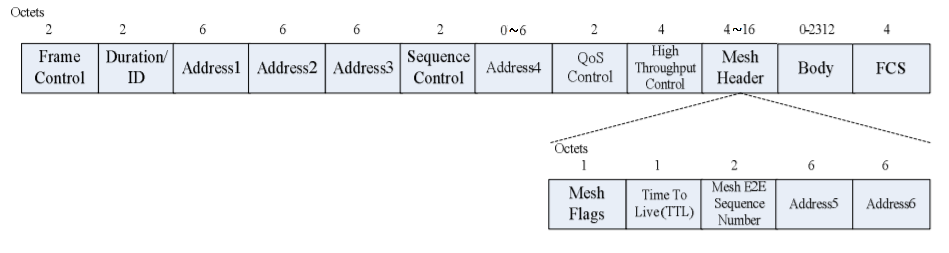
\includegraphics[width=\textwidth]{sensores/figuras/ele_pc2_du_02}
\caption{Quadro de comunicação IEEE 802.11s. Adaptada de:\cite{bib_ele_du_2}}
\label{ele_pc2_du_02}
\end{figure}

O quadro de comunicação também conta com um campo de mensagem que é definido como Mesh Header, responsável por organizar a distribuição de mensagens dentro da malha, controlando desde a inundação de transmissão de dados, através do ``Mesh e2e Sequence Number'', até evitar que dados da malha caiam acidentalmente em um \emph{loop} de encaminhamento infinito, através do TTL (\emph{Time To Live}).

Parte dos bits de \emph{Payload} do pacote padrão já gerado pelo transceptor (figura \ref{com_pc2_03}) devem ser utilizados para que se implemente o quadro de comunicação da rede \emph{mesh}. Assim, dos 32 \emph{bytes} disponíveis para envio de mensagem, 8 deles serão reservados para o envio informações referentes ao estabelecimento da malha. Os primeiros 2 \emph{bytes} são um identificador para a central da rede, outros 2 \emph{bytes} identificam o nó de origem da mensagem e os últimos 4 \emph{bytes} são uma \emph{timestamp} que indicam o horário de coleta dos dados no pacote.

A tabela \ref{tab_ele_gab_04} informa a quantidade de \emph{bits} necessários para a representação de cada um dos valores que devem ser transmitidos entre os nós da rede. Cada envio totaliza um total de 108 bits, o que pode ser enviado em apenas um pacote de dados. Outras informações importantes ao projeto estão contidas nesta mesma tabela, tais como os pinos necessários e o volume total de dados gerado em um dia, visto as 12 medições que são feitas ao longo deste período   

\begin{table}[H]
\caption{Volume de informações gerado por cada sensor}
\label{tab_ele_gab_04}
\begin{miniscule}
\begin{tabular}{cccc|c|c|c|c|c|c|}
\hline
\multicolumn{1}{|c|}{Medida} & \multicolumn{1}{c|}{\begin{tabular}[c]{@{}c@{}}Valores\\  Esperados\end{tabular}} & \multicolumn{1}{c|}{\begin{tabular}[c]{@{}c@{}}Mínima\\  Variação\end{tabular}} & Unidade & \begin{tabular}[c]{@{}c@{}}Tipo da\\  variável\end{tabular} & \begin{tabular}[c]{@{}c@{}}Quantidade \\ de bits\\  (Mínima)\end{tabular} & \begin{tabular}[c]{@{}c@{}}Envios\\  por dia\end{tabular} & \begin{tabular}[c]{@{}c@{}}Total de\\  bits por\\  dia\end{tabular} & \begin{tabular}[c]{@{}c@{}}Pinos\\ Analógicos\end{tabular} & \begin{tabular}[c]{@{}c@{}}Pinos\\  Digitais\end{tabular} \\ \hline
\multicolumn{1}{|c|}{Umidade do ar} & \multicolumn{1}{c|}{0  - 100} & \multicolumn{1}{c|}{0,008} & $\%$ & float & 16 & 12 & 192 & 0 & \multirow{4}{*}{2} \\ \cline{1-9}
\multicolumn{1}{|c|}{\begin{tabular}[c]{@{}c@{}}Temperatura\\  ambiente\end{tabular}} & \multicolumn{1}{c|}{0  - 60} & \multicolumn{1}{c|}{0,01} & $^{\circ}C$ & float & 16 & 12 & 192 & 0 &  \\ \cline{1-9}
\multicolumn{1}{|c|}{\begin{tabular}[c]{@{}c@{}}Pressão\\  atmosférica\end{tabular}} & \multicolumn{1}{c|}{300 - 1100} & \multicolumn{1}{c|}{0.18} & $hPa$ & float & 16 & 12 & 192 & 0 &  \\ \cline{1-9}
\multicolumn{1}{|c|}{Radição Solar} & \multicolumn{1}{c|}{} & \multicolumn{1}{c|}{0,01} & $W/m^2$ & float & 16 & 12 & 192 & 0 &  \\ \hline
\multicolumn{1}{|c|}{\begin{tabular}[c]{@{}c@{}}Umidade \\ do solo\end{tabular}} & \multicolumn{1}{c|}{0 - 100} & \multicolumn{1}{c|}{0,1} & $\%$ & float & 16 & 12 & 192 & 3 & 0 \\ \hline
\multicolumn{1}{|c|}{\begin{tabular}[c]{@{}c@{}}Temperatura \\ do solo\end{tabular}} & \multicolumn{1}{c|}{0 - 60} & \multicolumn{1}{c|}{0,1} & $^{\circ}C$ & float & 16 & 12 & 192 & 1 & 0 \\ \hline
\multicolumn{1}{|c|}{\begin{tabular}[c]{@{}c@{}}Velocidade\\  do vento\end{tabular}} & \multicolumn{1}{c|}{0 -  27} & \multicolumn{1}{c|}{0.1} & $m/s$ & float & 16 & 12 & 192 & 0 & 1 \\ \hline
\multicolumn{1}{|c|}{\begin{tabular}[c]{@{}c@{}}Direção\\  do vento\end{tabular}} & \multicolumn{1}{c|}{0 - 360} & \multicolumn{1}{c|}{1} & $^{\circ}$ & uint & 9 & 12 & 108 & 1 & 0 \\ \hline
\multicolumn{1}{|c|}{Pluviosidade} & \multicolumn{1}{c|}{0 -  200} & \multicolumn{1}{c|}{0.2} & $mm$ & uint & 8 & 12 & 96 & 0 & 1 \\ \hline
 &  &  &  & Total & 129 & 108 & 1548 & 5 & 4 \\ \cline{5-10} 
\end{tabular}
\end{miniscule}
\end{table}


Para garantir a funcionalidade da rede \emph{mesh}, além do quadro de comunicação é importante definir o sistema de rede de roteamento a ser utilizado. São possíveis os seguintes sistemas \cite{bib_ele_du_3}:

\begin{itemize}
	\item pró-ativos: os nós mantêm a informação da rota de todos os possíveis destinos, através de uma tabela de roteamento. Quando houver necessidade, a rota a ser utilizada será conhecida previamente.
	\item reativos:  não calculam as rotas a priori, sendo esta calculada apenas quando existe a necessidade de envio de mensagens.
	\item híbridos:  apenas alguns nós específicos atualizam periódicamente as rotas, enquanto outros continuam sendo reativos.
\end{itemize}

A baixa dinamicidade na malha de comunicação cria um ambiente ideal para redes pró-ativas, que para redes muito dinâmicas acabam gerando um fluxo de dados de controle muito alto, mas funciona com uma pequena taxa de perda de pacote e de poucos dados de controle para redes pouco voláteis a pequenas taxas de transmissão. Dentre os protocolos pró-ativos destaca-se o DSDV(\emph{Destination-Sequenced Distance-Vector}), baseado no algoritmo \emph{Distance Vector} de Bellman Ford. Tal método já foi usado em várias comparações, que mostram resultados mistos, mas seus resultados são especialmente bons para redes com variações lentas na topologia.\cite{bib_ele_du_6}

O DSDV é um protocolo de roteamento orientado por tabela, ou seja, cada nó mantém uma tabela de roteamento atualizada periodicamente com informações sobre a topologia da rede. Desse modo, quando há requisição de troca de mensagens, o caminho para chegar ao destino final seja conhecido automaticamente \cite{bib_ele_du_3}.Neste protocolo, todos os nós enviam informações aos demais por broadcast para o cálculo da tabela de roteamento. Na tabela contém a rota para cada nó na rede e a quantidade de saltos necessários para atingir cada destino. Em caso da perda de um determinado \emph{link}, os nós que perceberem essa alteração atualizam a tabela de roteamento e propagam essa informação aos demais, tornando a malha adaptativa.


A Figura \ref{ele_pc2_du_03} mostra a propagação de mensagens de controle entre os nós no momento do cálculo da tabela de roteamento.


\begin{figure}[H]
\centering
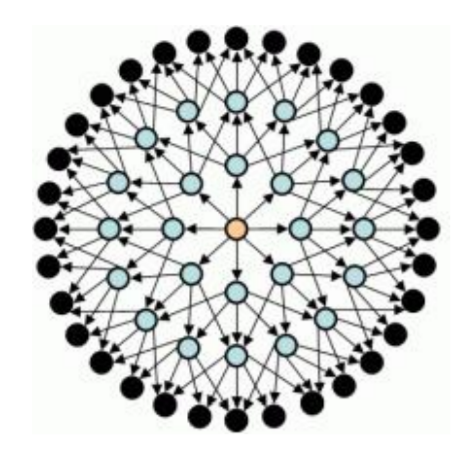
\includegraphics[width=.5\textwidth]{sensores/figuras/ele_pc2_du_03}
\caption{Propagação de mensagem por inundação. Fonte:\cite{bib_ele_du_3}}
\label{ele_pc2_du_03}
\end{figure}

A tabela de roteamento calculada possui informações sobre o caminho até cada destino possível, com o nó vizinho a que deve ser encaminhada a mensagem, a quantidade de saltos necessários até o destino e número de identidade do destino. Abaixo, um exemplo de uma tabela de roteamento DSDV.


\begin{figure}[H]
\centering
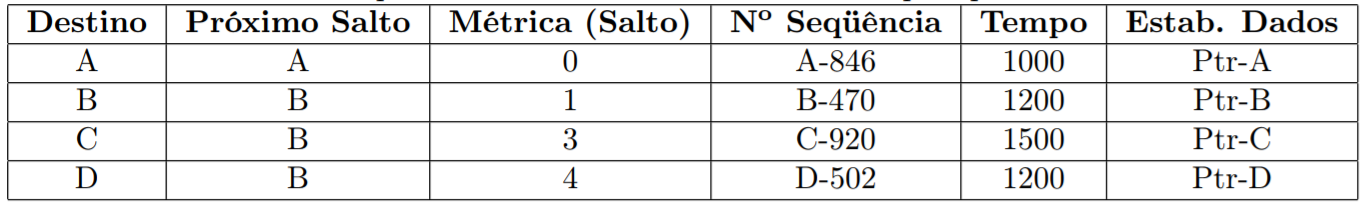
\includegraphics[width=\textwidth]{sensores/figuras/ele_pc2_du_04}
\caption{Exemplo de tabela de roteamento DSDV. Fonte:\cite{bib_ele_du_3}}
\label{ele_pc2_du_04}
\end{figure}

\section{Processamento}
		
	Cada um dos módulos que compõem o sistema possui funções específicas, de forma que o \emph{hardware} para cada um deles precisa de ser avaliado individualmente. No processo de escolha, deve-se considerar os circuitos periféricos que interfaceiam com a unidade de processamento a ser definida. Em comum, estações, central e atuadores devem possuir uma capacidade de processamento que os habilite a comunicar com o transceptor nRF24L01p (via I2C ou SPI) e executar os algoritmos de protocolo adicionais para a implementação da rede \emph{mesh}. A seguir são descritas as características particulares de cada um dos módulos:

	\begin{itemize}
		\item Estação:
			\begin{itemize}
				\item Capacidade de interfacear com todos os sensores estipulados (5 pinos digitas e 2 conversores A/D e 2 pinos para comunicação SPI).
				\item Capacidade de armazenar localmente todas as medidas ao longo de um dia (X bits).
			\end{itemize}
		\item Central:
			\begin{itemize}
				\item Possibilidade de estabelecer conexão estável com internet para realizar comunicação com os serviços em nuvem. 
				\item Memória suficiente para armazenar os dados de X estações por X dias (X bits)
			\end{itemize}
		\item Atuador:
			\begin{itemize}
				\item Capacidade de receber e executar os comandos para acionamento da carga.
			\end{itemize}
	\end{itemize}

	Dentre dez possíveis componentes disponíveis no mercado brasileiro, foram analisadas as seguintes características técnicas para a escolha daquele que melhor supra as necessidades do projeto: (i) memória RAM; (ii) memória para armazenamento de programa, (iii) quantidade de pinos digitais disponíveis para uso geral, (iv) quantidade de conversores A/D e (v) sua resolução; suporte nativo aos protocolos (vi) SPI, (vii) I2C e (viii) Wi-Fi de comunicação; (ix) \emph{clock} de processamento; (x) tensão de operação, (xi) corrente máxima drenada e (xii) preço. A tabela \ref{tab_ele_vic_01} resume tais informações, uma vez que todas os processadores possuem comunicação SPI e I2C, esta informação foi omitida da tabela.  


	\begin{table}[H]
		\centering
		\caption{Características avaliadas dos possíveis microcontroladores}
		\label{tab_ele_vic_01}
		\begin{miniscule}
			\begin{tabular}{|c|c|c|c|c|c|c|c|c|c|c|}
			\hline
			\multirow{2}{*}{Processador} & \multirow{2}{*}{\begin{tabular}[c]{@{}c@{}}SRAM \\ (Kb)\end{tabular}} & \multirow{2}{*}{\begin{tabular}[c]{@{}c@{}}Memória de\\  Programa\\  (Kb)\end{tabular}} & \multirow{2}{*}{\begin{tabular}[c]{@{}c@{}}GPIO\\ (Un)\end{tabular}} & \multicolumn{2}{c|}{\begin{tabular}[c]{@{}c@{}}Conversores\\  A/D\end{tabular}} & \multirow{2}{*}{\begin{tabular}[c]{@{}c@{}}Clock\\ (MHz)\end{tabular}} & \multirow{2}{*}{\begin{tabular}[c]{@{}c@{}}Corrente\\ (mA)\end{tabular}} & \multirow{2}{*}{\begin{tabular}[c]{@{}c@{}}Tensão\\ (V)\end{tabular}} & \multirow{2}{*}{Wi-Fi} & \multirow{2}{*}{\begin{tabular}[c]{@{}c@{}}Preço\\ \\ (R\$)\end{tabular}} \\ \cline{5-6}
			 &  &  &  & Qtd. & \begin{tabular}[c]{@{}c@{}}Resolução\\ (bits)\end{tabular} &  &  &  &  &  \\ \hline
			Raspberry Pi 3 B+ & 1000000 & 4000000 & 26 & 0 & - & 1400 & 230 & 5 & Sim & 200 \\ \hline
			Raspberry Pi Zero & 512000 & 4000000 & 26 & 0 & - & 1000 & 140 & 5 & Sim & 110 \\ \hline
			ESP32 & 520 & 448 & 40 & 20 & 12 & 240 & 80 & 4.5 $\sim$9 & Sim & 40 \\ \hline
			ESP8266 & 80 & 512 & 16 & 1 & 10 & 80 & 80 & 4.5 $\sim$9 & Sim & 22.96 \\ \hline
			MSP4302553G & 0.5 & 16 & 24 & 8 & 10 & 16 & 0.23 & 1.8 $\sim$3.6 & Não & 30 \\ \hline
			ATMEGA328P & 2 & 32 & 32 & 6 & 10 & 16 & 6.6 & 1.8 $\sim$5.5 & Não & 25 \\ \hline
			ATMEGA8A-PU & 1 & 8 & 23 & 6 & 10 & 16 & 3.6 & 2.7 $\sim$5.5 & Não & 14.8 \\ \hline
			PIC16F877A & 0.368 & 14.3 & 33 & 8 & 10 & 20 & 0.8 & 2 $\sim$5.5 & Não & 28.62 \\ \hline
			PIC18F452 & 1.5 & 32 & 34 & 8 & 10 & 40 & 1.6 & 2 $\sim$5.5 & Não & 38.88 \\ \hline
			PIC24FJ64GB002 & 8 & 64 & 34 & 9 & 10 & 32 & 10 & 2 $\sim$3.6 & Não & 35.45 \\ \hline
			\end{tabular}
		\end{miniscule}
	\end{table}

	\subsection{Processador da estação}

	Com os dados contidos na tabela \ref{tab_ele_vic_01} e as características desejadas para os processadores do sistema, construiu-se um quadro de decisão para cada um dos três diferentes módulos. Foi atribuída uma nota (1, 2, 4, 6, 8 ou 10) para cada um dos critérios. A nota dada é tão maior quanto a conformidade do processador para o requisito em análise. Além dos requisitos técnicos, foi adicionado o critério ``Facilidade de programação" que envolve os conhecimentos prévios da equipe com o processador em análise e a necessidade de aquisição \emph{hardware} específico para programação do componente (\emph{Pickit 3} para os microcontroladores da família PIC e a \emph{launchpad} para os da família MSP, nos valores de R\$ 76,90 e R\$ 92,00, respectivamente)

	\begin{table}[H]
		\caption{Matriz de decisão para processador da estação}
		\label{tab_ele_gab_01}
		\begin{tiny}

			\begin{tabular}{|c|c|c|c|c|c|c|c|c|}
				\hline
				Processador & SRAM & \begin{tabular}[c]{@{}c@{}}Memória\\ de Programa\end{tabular} & \begin{tabular}[c]{@{}c@{}}Resolução\\  do A/D\end{tabular} & Clock & Potência & Preço & \begin{tabular}[c]{@{}c@{}}Facilidade de\\ programação\end{tabular} & Total \\ \hline
				ESP32 & 10 & 10 & 10 & 10 & 2 & 6 & 10 & 58 \\ \hline
				MSP4302553G & 2 & 10 & 8 & 8 & 10 & 6 & 8 & 52 \\ \hline
				ATMEGA328P & 6 & 10 & 8 & 8 & 6 & 8 & 10 & 56 \\ \hline
				ATMEGA8A-PU & 4 & 8 & 8 & 8 & 6 & 10 & 10 & 54 \\ \hline
				PIC16F877A & 1 & 8 & 8 & 10 & 8 & 6 & 6 & 47 \\ \hline
				PIC18F452 & 4 & 10 & 8 & 10 & 8 & 6 & 6 & 52 \\ \hline
				PIC24FJ64GB002 & 10 & 10 & 8 & 10 & 6 & 6 & 6 & 56 \\ \hline

			\end{tabular}
		\end{tiny}
	\end{table}


	Foram desconsiderados da matriz de decisão as placas Raspberry Pi 3 B+, Raspberry Pi Zero devido ao elevado valor frente às demais possibilidades, a placa ESP8266 também foi desconsiderada por não atender a quantidade mínima de conversores A/D necessários. A maior pontuação foi atingida pelo microprocessador ESP32, suas principais qualidades são: (i) memória RAM e (ii) de armazenamento de programa, (ii) maior \emph{clock} de processamento e (iv) resolução dos conversores A/D. 

	\subsection{Processador do atuador}

	Uma segunda matriz de decisão foi elaborada para o processador dos atuadores. Aqui, a placa ESP8266 volta a ser uma possibilidade, visto que as entradas analógicas não são necessárias neste módulo do sistema. O processador do atuador deve interfacear somente com o transceptor e com o módulo relé, o que demanda apenas pinos digitais. Assim, a coluna referente à resolução do conversor A/D foi retirada. Também, como não será executada a aquisição de dados com os sensores, sua demanda de processamento é reduzida em relação à estação. Desde modo, as colunas referentes ao $clock$ e memória de programa não são mais consideradas na matriz de decisão, pois todas as opções possuem características mínimas nesses quesitos. Por fim, como o consumo de potência é um fator menos crítico no caso do atuador (dado sua forma de alimentação), os processadores em análise tiveram suas notas aumentadas neste quesito. As demais colunas, preço e facilidade de programação, mantiveram-se iguais.
	
\begin{table}[H]
\centering
\caption{Matriz de decisão para processador do atuador}
\label{tab_ele_gab_03}
\begin{tabular}{|c|c|c|c|c|c|}
\hline
Processador & SRAM & Potência & Preço & \begin{tabular}[c]{@{}c@{}}Facilidade de\\ programação\end{tabular} & Total \\ \hline
ESP32 & 10 & 6 & 6 & 10 & 42 \\ \hline
ESP8266 & 10 & 6 & 8 & 10 & 44 \\ \hline
MSP4302553G & 2 & 10 & 6 & 8 & 34 \\ \hline
ATMEGA328P & 6 & 8 & 8 & 10 & 40 \\ \hline
ATMEGA8A-PU & 4 & 8 & 10 & 10 & 40 \\ \hline
PIC16F877A & 1 & 10 & 6 & 6 & 33 \\ \hline
PIC18F452 & 4  & 10 & 6 & 6 & 36 \\ \hline
PIC24FJ64GB002 & 10 & 8 & 6 & 6 & 40 \\ \hline
\end{tabular}
\end{table}	

A tabela \ref{tab_ele_gab_03} apresenta a matriz de decisão para a escolha do processador dos atuadores. A melhor pontuação foi atingida pelo ESP8266 e a ESP32 (microprocessador escolhido para as estações) ficou em segundo lugar com apenas dois pontos de diferença. Pensando em um produto comercial, a padronização dos microcontroladores para todo o sistema se torna uma solução interessante visando economizar com pedidos em larga escala, especialmente considerando que as estações são, normalmente, mais numerosas do que os atuadores. Essa economia na compra pode compensar a diferença de preço entre os microcontroladores, fator decisivo na pontuação final da matriz de decisão. Por esse motivo, optou-se por também utilizar o ESP32 nos atuadores.

\subsection{Processador da central}

O módulo da central, diferentemente das estações e atuadores, não se comunicará apenas com a rede \emph{mesh}, mas também com o servidor central da aplicação. De acordo com a definição do produto, a central deve ser capaz de armazenar todos os dados coletados pelas estações e enviá-los para a aplicação, onde o usuário poderá acessá-los. Além disso, também deve receber informações do servidor, como as configurações de irrigação e a localização das estações, a qual deve ser inserida pelo operário por meio do aplicativo.

Dentre as formas de conexão entre a central e o servidor, foram avaliados, inicialmente, o uso dos serviços do próprio agricultor em sua fazenda, como conexões cabeadas de internet (\emph{Ethernet}) ou conexões sem fio (\emph{Wi-fi}) locais. Entretanto, tendo em vista o maior alcance de redes móveis, também foram analisados os serviços de GSM, GPRS e 3G. 

A vantagem de usar serviços móveis está em não demandar do cliente um acesso próprio, permitindo uma maior acessibilidade ao produto. Contudo, nesse caso, ainda seria necessário um chip SIM, envolvendo então uma mensalidade. Entre os serviço de GPRS e GSM, o primeiro apresenta funcionalidade mais interessantes para a proposta, considerando que já trabalha em pacotes de dados e alcança maiores taxas de transmissão. Já a rede 3G apresenta a maior taxa de transmissão entre as três, porém, é a que apresenta menor cobertura em áreas rurais.

Considerando os clientes que já possuem internet própria em algum lugar da fazenda, a rede \emph{Mesh} permitiria a entrega dos dados coletados de pontos mais distantes para o local conectado, contando que hajam nós suficientes entre eles e que a distância entre os nós não exceda os limites do módulo de comunicação. Neste caso, aproveitar a rede local se mostra mais vantajoso, considerando que o uso de redes móvel requer hardware adicional na central, como um módulo Sim800l para o GPRS, que custa na faixa de $R\$40,00$, além de um chip SIM e um plano de telefonia. Já para o acesso à redes locais, funcionalidades de acesso à internet são comumente disponíveis em SoCs (\emph{Systems on chip}), como na ESP32 ou na Raspberry Pi, podendo ser aproveitadas.

Segundo a matéria do jornal Valor Econômico \cite{bib_proc_vic_02}, uma pesquisa envolvendo três mil produtores realizada pela empresa Strider (empresa de tecnologias para o agronegócio), aponta que mais de $50\%$ das fazendas, independente do tamanho, possuem acesso à internet em pelo menos um lugar. Essa porcentagem aumenta de acordo com o tamanho da fazenda chegando perto de $100\%$ para fazendas de grande porte que são o público-alvo do produto, como pode ser observado no gráfico da figura \ref{ele_prc_vic_01}.

\begin{figure}
	\centering
	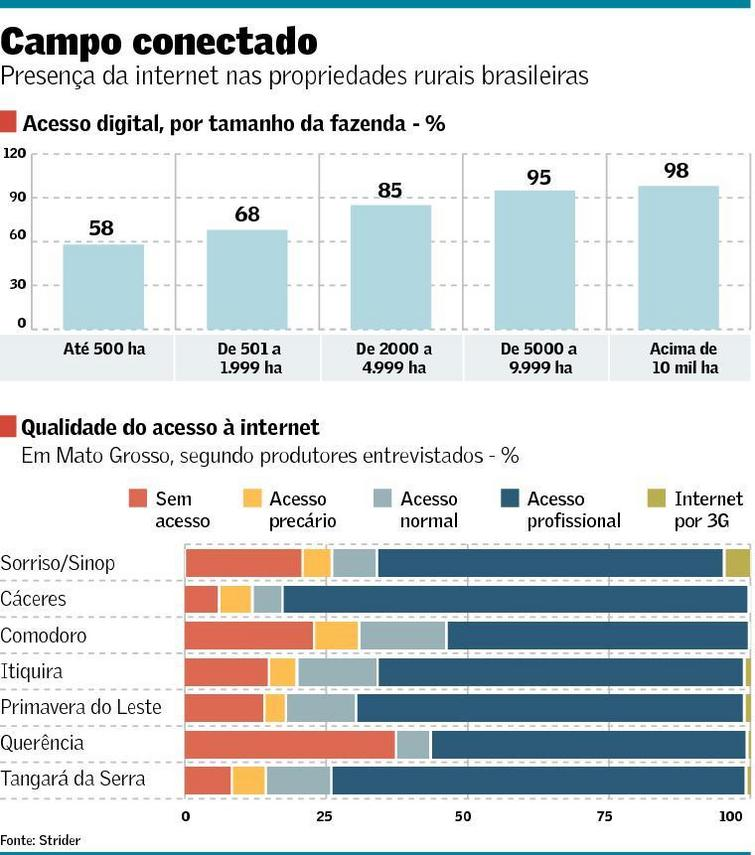
\includegraphics[width = 0.6\textwidth]{sensores/figuras/pro_sen_01}
	\caption{Sensor 034B. Fonte: \cite{bib_proc_vic_02}}
	\label{ele_prc_vic_01}
\end{figure}

Levando em consideranção que serviços de telefonia móvel sofrem constantes alterações, mudando de uma geração para outra, e que isso envolve também uma substituição do \emph{hardware}, o uso de um módulo como GPRS apresenta um risco potencial de perder o suporte e parar de funcionar, o que demandaria uma troca de todos os módulos centrais distribuídos. Essa situação não ocorre para o uso de internet local, onde melhorias do \emph{hardware} são de responsabilidade do cliente e não afetaria o funcionamento do sistema RICC. 

Portanto, olhando para o produto em longo prazo, o uso de redes locais promove uma maior facilidade tanto para a empresa quanto para o cliente e se mostra mais vantajoso em relação as outras alternativas. Por esses motivos, foi escolhido pelo uso da internet própria do cliente para a conexão com o servidor. A próxima etapa, é a escolha entre o uso de uma rede cabeada ou sem fio.

De acordo com o Núcleo de Informação e Coordenação do Ponto BR (órgão ligado ao Comitê Gestor da Internet no Brasil), aproximadamente 79\% da população rural que acessa a internet possui acesso com conexão cabeada \cite{bib_sen_gab_03}. Esse é um dado importante na decisão da forma de conexão com a internet. 

A desvantagem de usar uma rede \emph{Wi-fi} neste caso, se dá pela necessidade de inserção do SSID (nome da rede) e senha do usuário. Dependendo do processador escolhido, esses dados devem ser inseridos no código de programa, o que implicaria em questões de segurança. Além disso, a conexão cabeada é mais abrangente e possui a característica \emph{plug and play}, não necessitando de uma reconfiguração sempre que a senha da rede fosse alterada. Assim, foi decidido pelo uso de conexões \emph{Ethernet} cabeadas.

Este tipo de conexão da central não expõe um endereço de IP público para cada módulo, porém nosso servidor estará em nuvem pública. Dessa forma a comunicação deve ser iniciada e mantida pelas centrais sob sua própria demanda (através de \emph{Websockets}) para o estabelecimento e manutenção da conexão; e \emph{Polling}, para requisições periódicas caso haja alguma interrupção. Tais funcionalidades demandam recursos de um sistema operacional.

A implementação do controle da conexão com a internet e utilização do protocolo HTTP envolve bastante complexidade de programação, principalmente se desenvolvida em linguagens de baixo nível como C. Outras soluções através de linguagens com maiores recursos de segurança e robustez não podem ser implementadas em microcontroladores comuns, dada a inviabilidade de execução de duas linguagens simultâneas.

Além disso, como conversado com o professor Bruno César Ribas (que ministra a disciplina de Fundamento de Sistemas Operacionais), gerenciar a conexão com a internet, stack TCP e enviar requisições HTTP, realizando paralelamente o processamento e recebimento dos dados da estação pela rede \emph{mesh}, é uma tarefa que demanda uma elevada capacidade de processamento do hardware. 

Ainda que possível a implementação desse sistema em um microcontrolador, como a ESP32 usada pelas estações, tal solução requer um nível de otimização de código e uma quantidade de testes e adaptações que inviabilizaria o desenvolvimento do projeto para o tempo da disciplina. Por esses motivos, optou-se pela utilização de um sistema operacional embarcado.

Nesta fase de prototipagem, a adoção da placa \emph{Raspberry Pi modelo 3B} como o \emph{hardware} para a central se mostra interessante, considerando a disponibilidade e conhecimento da placa pelo grupo. Suas especificações foram listadas anteriormente na tabela \ref{}. Além do preço, que para o protótipo não é relevante (considerando que o grupo já a possui), sua outra desvantagem é o consumo energético. Entretanto, como a central estará conectada com a rede elétrica da fazenda, este quesito passa a ser menos prejudicial ao produto. Assim, a placa Raspberry Pi modelo 3B foi escolhida como o processador para a central.

\section{Funcionamento geral do sistema eletrônico}

	\subsection{Diagrama de blocos do sistema eletrônico}

	\subsection{Diagrama lógico do sistema eletrônico}

	\subsection{Controle da irrigação}

\section{Esquemáticos dos circuitos}
	Uma vez que foram definidos todos os componentes e circuitos eletrônicos necessários, seus comportamentos esperados e fluxos de dados entre as partes, pode-se elaborar suas conexões físicas. A seguir são mostrados os esquemáticos dos circuitos para cada um dos módulos do sistema, bem como projetos preliminares das placas de circuito impresso.
	
	
	\subsection{Estação}
Os circuitos da estação ficarão concentrados em uma única placa, que abrigará o microcontrolador  e os circuitos de condicionamento para os sensores de temperatura do solo e direção do vento.  Os sensores e o módulo transceptor possuem posições específicas ao longo da estação (conforme mostrado na descrição da estrutura). Tais componentes interfacearão  com a placa principal por meio de conectores e cabeamento. 


A ESP32 é acoplada a placa por meio de um soquete, para que facilite a troca em caso de defeito e possibilita também o aproveitamento deste componente em outros projetos. As ligações necessárias entre pinos são feitas por meio das trilhas impressas na placa. A figura \ref{ele_pc2_gab_03} indica os pinos utilizados do microcontrolador, que desempenham as funções de comunicação SPI e I2C (com o transceptor e o sensor BME280) e interface com os sensores.  

\begin{figure}[H]
	\centering
%	\includegraphics[]{sensores/figuras/ele_pc2_gab_03}
	\caption{Ligação dos pinos no microcontrolador}
	\label{ele_pc2_gab_03}
\end{figure}

Por fim, a partir do esquemático completo, apresentado ao fim deste relatório em anexo, foi elaborado o \emph{layout} da placa de circuito impresso, onde pode-se observar as trilhas, o posicionamento de todos os componentes, entre soquetes, conectores e circuitos auxiliares de condicionamento. O desenho da placa é apresentado na figura \ref{ele_pc2_gab_04}.


\begin{figure}[H]
	\centering
%	\includegraphics[]{sensores/figuras/ele_pc2_gab_04}
	\caption{\emph{Layout} da placa de circuito impresso para estação}
	\label{ele_pc2_gab_04}
\end{figure}		


	\subsection{Central}
	O circuito presente na central é mais simples comparado ao existente nas estações. Este circuito é composto por dois componentes: (i) \emph{Raspberry Pi 3B} e (ii) transceptor nRF24L01p. As conexões possibilitam a comunicação SPI entre estas duas partes e o controle do funcionamento transceptor pela \emph{Raspberry Pi}. A figura \ref{ele_pc2_gab_05} mostra tais ligações.

\begin{figure}[H]
	\centering
%	\includegraphics[]{sensores/figuras/ele_pc2_gab_05}
	\caption{Esquemático do circuito da central}
	\label{ele_pc2_gab_05}
\end{figure}		

A implementação deste circuíto consiste da fabricação de um \emph{shield}, cujo \emph{layout}  é mostrado na figura \ref{ele_pc2_gab_06}
	
	\begin{figure}[H]
		\centering
   %	\includegraphics[]{sensores/figuras/ele_pc2_gab_06}
		\caption{\emph{Layout} da placa de circuito impresso para central}
		\label{ele_pc2_gab_06}
\end{figure}		

		

	\subsection{Atuador}


O circuito dos atuadores também concentra-se em uma única placa, que abriga o microcontrolador e possibilita sua interface com o módulo transceptor  e o módulo relé para acionamento da carga. Novamente, a ESP32 é acoplada à placa por meio de um soquete e as ligações necessárias entre pinos são feitas por meio das trilhas impressas na placa. O esquemático deste circuito é  apresentado na figura \ref{ele_pc2_gab_07} 

\begin{figure}[H]
	\centering
%	\includegraphics[]{sensores/figuras/ele_pc2_gab_07}
	\caption{Esquemático do circuito do atuador}
	\label{ele_pc2_gab_07}
\end{figure}

O projeto da placa de circuito impresso partiu de modificações no projeto da placa das estações, vistos que os circuitos apresentam semelhanças (ligações entre controlador e módulo de comunicação). O desenho da placa é apresentado na figura \ref{ele_pc2_gab_08}.

\begin{figure}[H]
	\centering
%	\includegraphics[]{sensores/figuras/ele_pc2_gab_08}
	\caption{Esquemático do circuito do atuador}
	\label{ele_pc2_gab_08}
\end{figure}


\begin{figure}[H]
	\centering
%	\includegraphics[]{sensores/figuras/ele_pc2_gab_04}
	\caption{\emph{Layout} da placa de circuito impresso para central}
	\label{ele_pc2_gab_04}
\end{figure}		



\section{Plano de construção}

	Estação
		
		- PCB
	
	Central
		
		- PCB
		
	Atuador
	
		- PCB

\section{Plano de teste}

	O sistema eletrônico do RICC, depois de construído, deve ser testado para que seja avaliado seu funcionamento. Os procedimentos a seguir descritos serão realizados com o objetivo de verificar a conformidade entre o sistema implementado e o projetado. Busca-se, assim, viabilizar a integração entre os subsistemas do produto. 

	\subsection{Teste do sistema de sensoriamento}
		Teste individual dos sensores:
			
			- Teste da saída dos sensores para mudanças forçadas no ambiente
			
			- Leitura da saída com o microcontrolador
		
		Teste conjunto dos sensores com o microcontrolador:
		
			- Leitura de todos os sensores e formação dos pacotes
			
			- Analise dos pacotes salvos
	
	\subsection{Teste do sistema de comunicação}
	
		Os custos para a construção de uma estação são elevados. Porém, são necessários alguns nós para a validação do funcionamento da rede \emph{mesh}. Desta forma, será feita apenas uma estação completa, com as partes estruturais e os sistemas de energia e de sensoriamento. Outras duas estações serão simuladas. O nó da central é único no sistema e também será construído. Por fim, também será implementado o sistema completo de um atuador. 
	
		As estações simuladas são compostas por um microcontrolador e um transceptor. Nelas, serão implementados os algoritmos de comunicação, mas os pacotes de dados (que seriam fornecidos pelos sensores) estarão previamente gravados na memória. Assim, a dinâmica da rede \emph{mesh} poderá ser verificada sem que sejam gastos recursos com a construção de outra estação completa.  
				
		Criação de pacotes de dados padrão para o teste da rede
		
		Teste da comunicação de um pacote entres diferentes nós 

		Teste da rede com vários pacotes a serem enviados para a central
		
		Teste da forma com que a central processa e armazena múltiplos dados
		
		
